\documentclass[12pt]{article}
\usepackage{a4wide, amsfonts, epsfig}
\newcommand\soln{\noindent\textit{Solution:} }


%skyline stuff
\font\upright=cmu10 scaled\magstep1
\setlength{\unitlength}{0.012500in}
\begingroup\makeatletter\ifx\SetFigFont\undefined
\def\x#1#2#3#4#5#6#7\relax{\def\x{#1#2#3#4#5#6}}%
\expandafter\x\fmtname xxxxxx\relax \def\y{splain}%
\ifx\x\y   % LaTeX or SliTeX?
\gdef\SetFigFont#1#2#3{%
  \ifnum #1<17\tiny\else \ifnum #1<20\small\else
  \ifnum #1<24\normalsize\else \ifnum #1<29\large\else
  \ifnum #1<34\Large\else \ifnum #1<41\LARGE\else
     \huge\fi\fi\fi\fi\fi\fi
  \csname #3\endcsname}%
\else
\gdef\SetFigFont#1#2#3{\begingroup
  \count@#1\relax \ifnum 25<\count@\count@25\fi
  \def\x{\endgroup\@setsize\SetFigFont{#2pt}}%
  \expandafter\x
    \csname \romannumeral\the\count@ pt\expandafter\endcsname
    \csname @\romannumeral\the\count@ pt\endcsname
  \csname #3\endcsname}%
\fi
\fi\endgroup

\begin{document}
\begin{center}
{\bf 2E2 Tutorial Sheet 11 Second Term, Solutions}\footnote{Conor
Houghton, {\tt houghton@maths.tcd.ie} and {\tt
http://www.maths.tcd.ie/\char126 houghton/ 2E2.html}}
\\[1cm]
 22 January 2006
\end{center}
\textsf{
\begin{enumerate}
\item (2) For the system
\begin{eqnarray*}
\frac{dy_1}{dt}&=&-3y_1+2y_2\\
\frac{dy_2}{dt}&=&-2y_1+2y_2
\end{eqnarray*}
The solution is
\begin{equation}
{\bf y}=c_1\left(\begin{array}{c}1\\2\end{array}\right)e^t+c_2\left(\begin{array}{c}2\\1\end{array}\right)e^{-2t}
\end{equation}
Sketch the phase diagram and and describe the stationary point.
\vskip .5cm
\soln So, any point that starts on the 
\begin{equation}
\left(\begin{array}{c}2\\1\end{array}\right)
\end{equation}
eigenvector will move inwards, since $c_1=0$ and $c^2\exp{-2t}$ gets
small as $t$ increases, anywhere on the other eigenvectors will move
straight outwards. If you aren't on either eigenvector, the amount along the negative eigenvalue eigenvector decreases and the amount along the positive eigenvector eigenvalue increases and so you move outwards getting closer and closer to the positive eigenvalue line.
The phase diagram is
\begin{center}
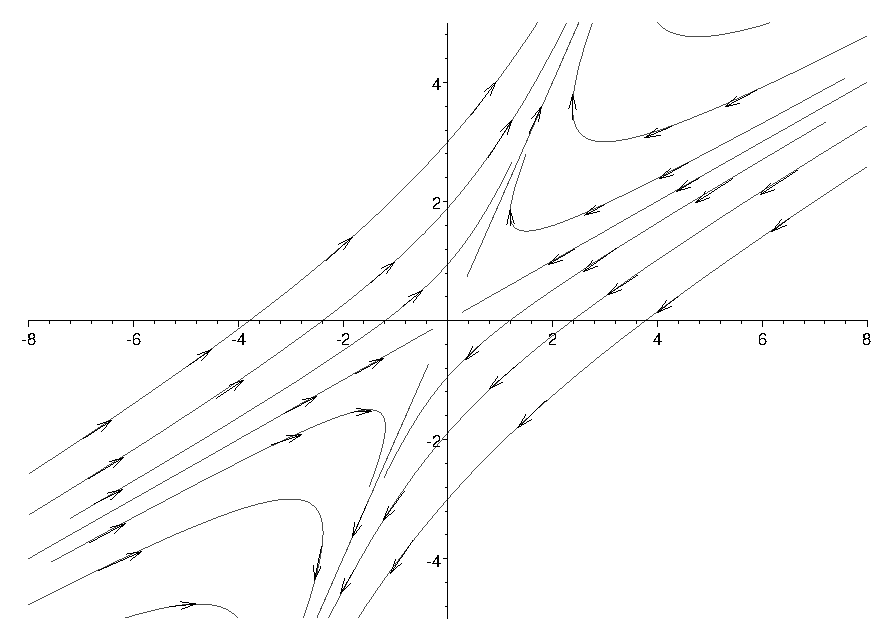
\epsfig{file=saddlearrowed.eps, width=10cm}
\end{center}
where the arrows go outwards except on the line defined by ${\bf
x}_2$.  The stationary point is a saddle point.
\vskip .5cm
\item (2) For the system
\begin{eqnarray}
\frac{dy_1}{dt}&=&3y_1+y_2\\
\frac{dy_2}{dt}&=&y_1+3y_2
\end{eqnarray}
The solution is 
\begin{equation}{\bf y}=\left(\begin{array}{cc}y_1\\y_2\end{array}\right)=c_1\left(\begin{array}{cc}1\\1\end{array}\right)e^{4t}+c_2\left(\begin{array}{cc}-1\\1\end{array}\right)e^{2t}.\end{equation}
Sketch the phase diagram and and describe the stationary point.
\vskip .5cm
\soln
The phase-diagram is 
\begin{center}
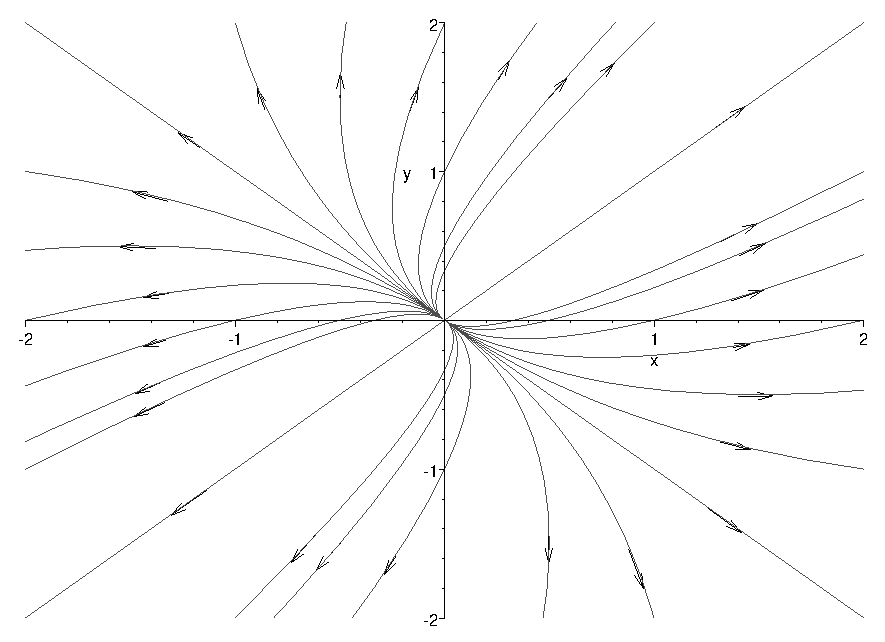
\epsfig{file=imnode2.eps,width=10cm}
\end{center}
with all the lines going outward. Notice they are all tending towards
the same direction as ${\bf x}_1$.
\vskip .5cm
\item (4) Find the general solutions for the system
\begin{eqnarray}
\frac{dy_1}{dt}&=&2y_1-y_2\\
\frac{dy_2}{dt}&=&-4y_2
\end{eqnarray}
Sketch the phase diagram and and describe the stationary point.
\vskip .5cm
\soln So here
$$A=\left(\begin{array}{cc}2&-1\\0&-4\end{array}\right)$$ and the
spectrum\footnote{The set of eigenvalues of a matrix is sometimes
called its spectrum} is $\lambda_1=2$ corresponding to
$${\bf x}_1=\left(\begin{array}{cc}1\\0\end{array}\right)$$
and $\lambda_2=-4$ corresponding to 
$${\bf x}_2=\left(\begin{array}{cc}1\\6\end{array}\right)$$
so the general solution is
$${\bf y}=\left(\begin{array}{cc}y_1\\y_2\end{array}\right)=c_1\left(\begin{array}{c}1\\0\end{array}\right)e^{2t}+c_2\left(\begin{array}{c}1\\6\end{array}\right)e^{-4t}.$$
The phase diagram is 
\begin{center}
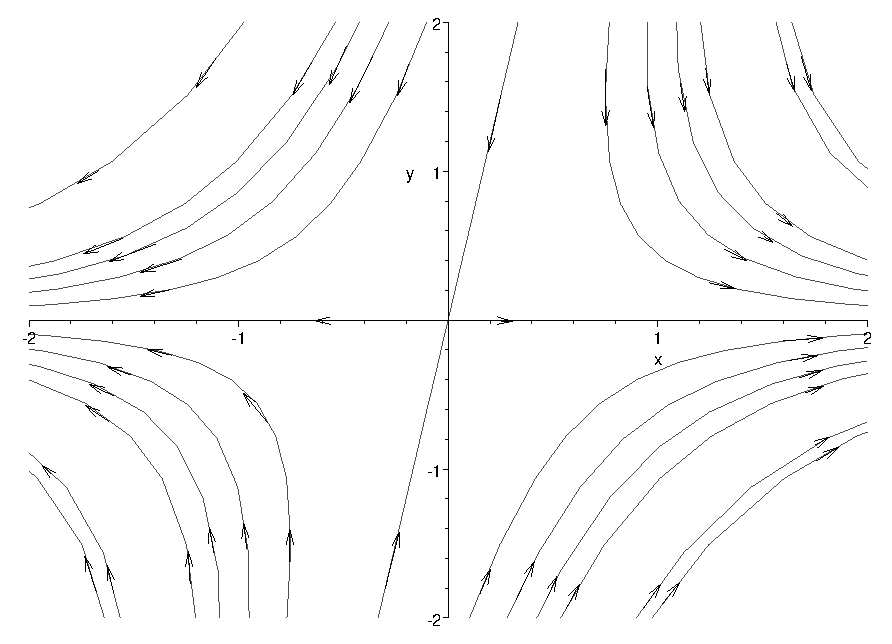
\epsfig{file=saddle2d.eps, width=10cm}
\end{center}
\end{enumerate}
}
\end{document}